\documentclass{article}

% if you need to pass options to natbib, use, e.g.:
%     \PassOptionsToPackage{numbers, compress}{natbib}
% before loading neurips_2020

% ready for submission
% \usepackage{neurips_2020}
\usepackage[final]{neurips_2020_ml4ps}
% to compile a preprint version, e.g., for submission to arXiv, add add the
% [preprint] option:
%     \usepackage[preprint]{neurips_2020}

% to compile a camera-ready version, add the [final] option, e.g.:
%     \usepackage[final]{neurips_2020}

% to avoid loading the natbib package, add option nonatbib:
%     \usepackage[nonatbib]{neurips_2020}

\usepackage[utf8]{inputenc} % allow utf-8 input
\usepackage[T1]{fontenc}    % use 8-bit T1 fonts
\usepackage{hyperref}       % hyperlinks
\usepackage{url}            % simple URL typesetting
\usepackage{booktabs}       % professional-quality tables
\usepackage{amsfonts}       % blackboard math symbols
\usepackage{nicefrac}       % compact symbols for 1/2, etc.
\usepackage{microtype}      % microtypography

\usepackage{amsmath}
\usepackage{graphicx}
\usepackage{enumerate}
\usepackage{natbib}
\usepackage{url}
\usepackage{enumitem}

\usepackage{amsmath,amssymb,amsthm,bm,mathtools}
\usepackage{algorithm}
\usepackage{dsfont,multirow,hyperref,setspace,enumerate}
\hypersetup{colorlinks,linkcolor={black},citecolor={black},urlcolor={black}}

\theoremstyle{definition}
\newtheorem{thm}{Theorem}[section]
\newtheorem{lem}{Lemma}
\newtheorem{prop}{Proposition}
\newtheorem{pro}{Property}
\newtheorem{cor}{Corollary}[section]

\theoremstyle{definition}
\newtheorem{assumption}{Assumption}
\newtheorem{defn}{Definition}
\newtheorem{example}{Example}
\newtheorem{rmk}{Remark}

\usepackage{appendix}
\usepackage{wrapfig}
\mathtoolsset{showonlyrefs}


\usepackage{algpseudocode,algorithm}
\algnewcommand\algorithmicinput{\textbf{Input:}}
\algnewcommand\algorithmicoutput{\textbf{Output:}}
\algnewcommand\INPUT{\item[\algorithmicinput]}
\algnewcommand\OUTPUT{\item[\algorithmicoutput]}




\usepackage{xr}

\input macros.tex


\title{Learning Multiple Networks via Supervised Tensor Decomposition}

% The \author macro works with any number of authors. There are two commands
% used to separate the names and addresses of multiple authors: \And and \AND.
%
% Using \And between authors leaves it to LaTeX to determine where to break the
% lines. Using \AND forces a line break at that point. So, if LaTeX puts 3 of 4
% authors names on the first line, and the last on the second line, try using
% \AND instead of \And before the third author name.

%\author{%}

\author{%
  Jiaxin Hu \\
  Department of Statistics\\
  University of Wisconsin-Madison\\
  Madison, WI 53706\\
  \texttt{jhu267@wisc.edu} \\
  
  \And
  Chanwoo Lee \\
  Department of Statistics\\
  University of Wisconsin-Madison\\
  Madison, WI 53706\\
  \texttt{chanwoo.lee@wisc.edu} \\
  
  \And
  
  Miaoyan Wang \\
  Department of Statistics\\
  University of Wisconsin-Madison\\
  Madison, WI 53706\\
  \texttt{miaoyan.wang@wisc.edu} \\

}


\begin{document}

\maketitle

\begin{abstract}
We consider the problem of tensor decomposition with multiple side information available as interactive features. Such problems are common in neuroimaging, network modeling, and spatial-temporal analysis. We develop a new family of exponential tensor decomposition models and establish the theoretical accuracy guarantees. An efficient alternating optimization algorithm is further developed. Unlike earlier methods, our proposal is able to handle a broad range of data types, including continuous, count, and binary observations. We apply the method to diffusion tensor imaging data from human connectome project and identify the key brain connectivity patterns associated with available features. Our method will help the practitioners efficiently analyze tensor datasets in various areas. Toward this end, all data and code have been made available to the public. 
\end{abstract}

\section{Introduction}
 Higher-order tensors have received increased attention across science and engineering. While most tensor decomposition methods are developed for a single tensor observation, scientific studies often collect side information, in the form of node features and interactions thereof, together with the tensor data. Such data problems are common in neuroimaging, network analysis, and spatial-temporal modeling. A popular example is in neuroimaging~\citep{zhou2013tensor}. The brain connectivity networks are collected from a sample of individuals, accompanied by individual characteristics such as age, gender, and diseases status (see Figure~\ref{fig:intro1}a). Another example is in network analysis~\citep{pmlr-v108-berthet20a}. Side information such as people’s demographic information and friendship types are often available. In both examples, scientists are interested in identifing the variation in the data tensor (e.g., brain connectivities, social community patterns) that is affected by available features. These seemingly different scenarios pose a common yet challenging problem for tensor data modeling. 
 
 \begin{figure}[hbt]
 \vspace{-.4cm}
\begin{center}
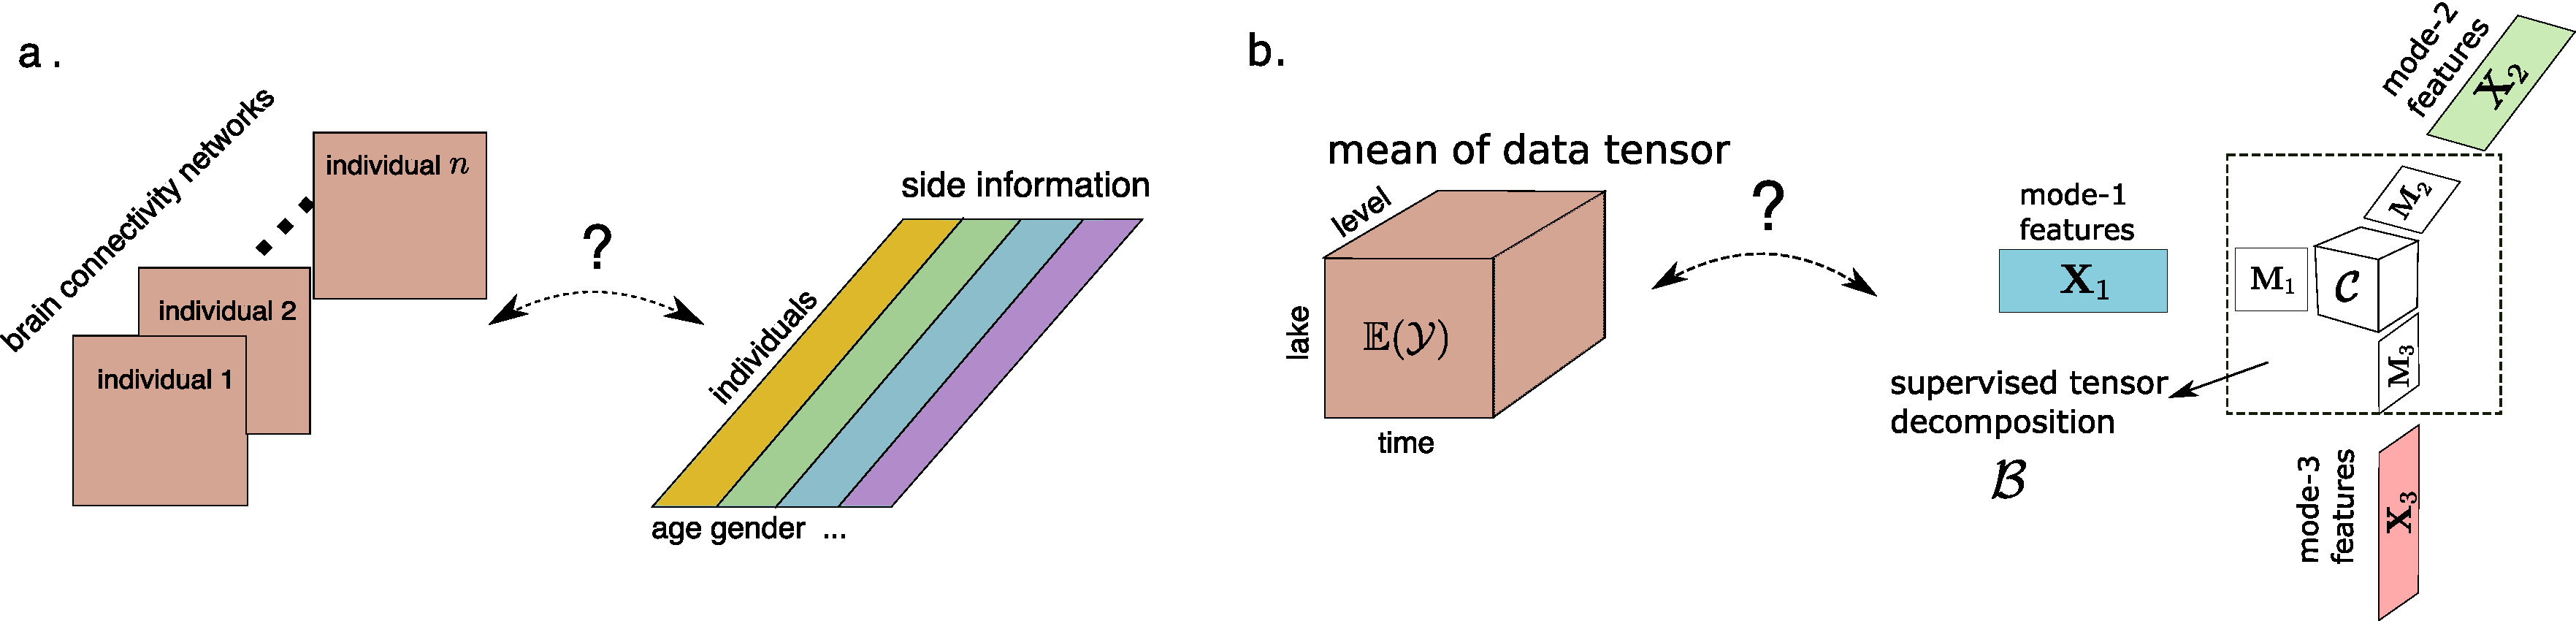
\includegraphics[width = 13.5cm]{demo.pdf}
\vspace{-.4cm}
\end{center}
\caption{Examples of supervised tensor decomposition with interactive side information. (a) Network population model. (b) Spatio-temporal growth model.} \label{fig:intro1}
\vspace{-.2cm}
\end{figure}

In addition to the challenge of incorporating side information, another challenge is that many tensor datasets consist of non-Gaussian measurements. Classical tensor decomposition methods are based on minimizing the Frobenius norm of deviation, leading to suboptimal predictions for binary- or count-valued response variables. A number of supervised tensor methods have been proposed \citep{narita2012tensor, zhao2012higher, yu2016learning,lock2018supervised}. These methods often assume Gaussian distribution for the tensor entries, or impose random designs for the feature matrices, both of which are less suitable for applications of our interest. We overcome those challenges from new modeling and narrow the gap between theory and practice.

{\bf Our contribution.} This paper presents a general model and associated method for decomposing a data tensor whose entries are from exponential family with interactive side information. We formulate the learning task as a low-rank tensor regression problem, with tensor observation serving as the response, and the multiple side information as interactive features. We blend the modeling power of generalized linear model (GLM) and the exploratory capability of tensor dimension reduction in order to take the best out of both sides. Our method greatly improves the classical tensor decomposition, and we quantify the improvement in prediction through numerical experiments and data applications. 

{\bf Notation.} We follow the tensor notation as in~\cite{kolda2009tensor}. The multilinear multiplication of a tensor $\tY\in\mathbb{R}^{d_1\times \cdots\times d_K}$ by matrices $\mX_k=\entry{x_{i_k,j_k}^{(k)}}\in\mathbb{R}^{p_k\times d_k}$ is defined as $\tY\times\{\mX_1,\ldots,\mX_K\} =\entry{\sum_{i_1,\ldots,i_K}y_{i_1,\ldots,i_K}x_{j_1,i_1}^{(1)}\cdots x_{j_K,i_K}^{(K)}}$,
which results in an order-$K$ $(p_1,\ldots,p_K)$-dimensional tensor. The inner product between two tensors of equal size is defined as $\langle \tY,\ \tY'\rangle =\sum_{i_1,\ldots,i_K}y_{i_1,\ldots,i_K}y'_{i_1,\ldots,i_K}$. For ease of notation, we allow basic arithmetic operators (e.g.,\ $+, -$) and univariate functions $f\colon \mathbb{R}\to \mathbb{R}$ to be applied to tensors in an element-wise manner. Besides, let $\otimes$ denote the Kronecker product of matrices.

\vspace{-0.2cm}
\section{Proposed models and motivating examples}
\vspace{-0.2cm}
%For any two matrices $\mA,\mB$ with orthonormal columns of same dimension, the angle distance is defined as
%\[ \sin \Theta(\mA,\mB)=\snormSize{}{\mA^T \mB^{\perp}}=\max\left\{ \frac{\langle \mx, \my\rangle}{\vnormSize{}{\mx}\vnormSize{}{\my}}\colon \ \mx\in \textup{Span}(\mA),\ \my\in \textup{Span}(\mB^\perp)\right\}. \]
Let $\tY=\entry{y_{i_1,\ldots,i_K}}\in\mathbb{R}^{d_1\times \cdots\times d_K}$ denote an order-$K$ data tensor. Suppose the side information is available on each of the $K$ modes. Let $\mX_k=\entry{x_{ij}}\in\mathbb{R}^{d_k\times p_k}$ denote the feature matrix on the mode $k\in[K]$, where $x_{ij}$ denotes the $j$-th feature value for the $i$-th tensor entity, for $(i,j)\in[d_k]\times[p_k]$, $p_k\leq d_k$. We assume that, conditional on the features $\mX_k$, the entries of tensor $\tY$ are independent realizations from an exponential family distribution, and the conditional mean tensor admits the form
\begin{align}\label{eq:decomp}
\mathbb{E}(\tY|\mX_1,\ldots,\mX_K) &= f\left(\tC\times\{\mX_1\mM_1, \ldots, \mX_K\mM_K\}\right),\notag\\
\text{with} \ &\ \mM_k^T\mM_k = \mI_{r_k},\ \mM_k\in\mathbb{R}^{p_k\times r_k}\quad \text{for all }k=1,\ldots,K.
\end{align}
where $\tC\in\mathbb{R}^{r_1\times \cdots \times r_K}$ is a full-rank core tensor, $\mM_k\in\mathbb{R}^{p_k\times r_k}$ are factor matrices consisting of orthonormal columns with $r_k\leq p_k$ for all $k\in[K]$, and $f(\cdot)$ is a known link function whose form depending on the data type of $\tY$. Common choices of link functions include identity link for Gaussian distribution, logistic link for Bernoulli distribution, and $\exp(\cdot)$ link for Poisson distribution. 

Figure~\ref{fig:intro1}b provides a schematic illustration of our model. The features $\mX_k$ affect the distribution of tensor entries in $\tY$ through the sufficient features of the form $\mX_k\mM_k$, which are $r_k$ linear combinations of features on mode $k$. The core tensor $\tC$ collects the interaction effects between sufficient features across $K$ modes, which links the conditional mean to the feature spaces, and thus allows the identification of variations in the tensor data attributable to the side information. Our goal is to find $\mM_k$ and the corresponding $\tC$ to reveal the relationship between side information $\mX_k$ and the observed tensor $\tY$. Note that $\mM_k$ and $\tC$ are identifiable only up to orthonormal transformations.  

We give two examples of supervised tensor decomposition models~\eqref{eq:decomp} that arise in practice.
\begin{example}[Spatio-temporal growth model]
The growth curve model~\citep{srivastava2008models} was originally proposed as an example of bilinear model for matrix data, and we extend it to higher-order cases. Let $\tY=\entry{y_{ijk}}\in\mathbb{R}^{d \times m\times n}$ denote the pH measurements of $d$ lakes at $m$ levels of depth and for $n$ time points. Suppose the sampled lakes belong to $q$ types, with $p$ lakes in each type. Let $\{\ell_j\}_{j\in[m]}$ denote the sampled depth levels and $\{t_k\}_{k\in[n]}$ the time points. Assume that the expected pH trend in depth is a polynomial of order at most $r$ and that the expected trend in time is a polynomial of order $s$. Then, the conditional mean model for the spatio-temporal growth is a special case of our model~\eqref{eq:decomp}, where $\mX_1=\text{blockdiag}\{\mathbf{1}_q,\ldots,\mathbf{1}_q\}\in \{0,1\}^{d\times p}$ is the design matrix for lake types, 
\[
\mX_2=
\begin{pmatrix}
1 & \ell_1&\cdots &\ell^{r}_1\\
1 & \ell_2&\cdots &\ell^{r}_2\\
\vdots &\vdots&\ddots&\vdots\\
1&\ell_{m}&\cdots&\ell^{r}_{m}
\end{pmatrix},\
\mX_3=
\begin{pmatrix}
1 & t_1&\cdots &t^{s}_1\\
1 & t_2&\cdots &t^{s}_2\\
\vdots &\vdots&\ddots&\vdots\\
1&t_{n}&\cdots&t^{s}_{n}
\end{pmatrix}
\]
are the design matrices for spatial and temporal effects, respectively. The spatial-temporal mode has covariates available on each of the three modes. 

\end{example}
\begin{example}[Network population model] 
Network response model is recently developed in the context of neuroimanig analysis. The goal is to study the relationship between network-valued response and the individual covariates. Suppose we observe $n$ i.i.d.\ observations $\{(\mY_i, \mx_i): i=1,\ldots,n\}$, where $\mY_i\in\{0,1\}^{d\times d}$ is the brain connectivity network on the $i$-th individual, and $\mx_i\in\mathbb{R}^p$ is the individual covariate such as age, gender, cognition, etc. The network-response model~\citep{rabusseau2016low} has the form
\begin{equation}\label{eq:network}
\text{logit}(\mathbb{E}(\mY_i|\mx_i))=\tB\times_3\mx_i, \quad \text{for }i=1,\ldots,n
\end{equation}
where $\tB\in \mathbb{R}^{d\times d\times p}$ is the coefficient tensor of interest. The model~\eqref{eq:network} is also a special case of our tensor-response model, with covariates on the last mode of the tensor. 
\end{example}

\vspace{-0.2cm}

\section{Estimation methods and theoretical results}

\vspace{-0.2cm}
We develop a likelihood-based procedure to estimate $\tC$ and $\mM_k$ in~\eqref{eq:decomp}. Ignoring constants that do not depend on $\Theta$, the quasi log-likelihood of~\eqref{eq:decomp} is equal to
\begin{equation}\label{eq:loglikelihood}
\small
\tL_{\tY}(\tC,\mM_1,\ldots,\mM_K)=\langle \tY, \Theta \rangle - \sum\nolimits_{i_1,\ldots,i_K} b(\theta_{i_1,\ldots,i_K})\ \text{with}\ \Theta=\tC\times\{\mM_1\mX_1,\ldots,\mM_K\mX_K\},
\end{equation}
where $b(\theta)=\theta^2/2$ for Gaussian response, $b(\theta)=\exp(\theta)$ for Poisson response, and $b(\theta)=\log(1+\exp(\theta))$ for Bernoulli response. We propose a constrained maximum quasi-likelihood estimator (M-estimator),
\begin{align} \label{eq:MLE} 
(\hat \tC, \hat \mM_1,\ldots,\hat \mM_k) &=\argmax_{(\tC,\mM_1,\ldots,\mM_K)\in \tP} \ \tL_{\tY}(\tC,\mM_1,\ldots,\mM_K),
\end{align}
where parameter space 
$
\tP=\left\{(\tC, \mM_1,\ldots,\mM_K) \ \Big| \ \mM_k^T\mM_k=\mathbf{I}_{r_k},\ \mnormSize{}{\Theta(\tC,\mM_1,\ldots,\mM_K)}\leq \alpha \right\}
$, and $\alpha$ is a constant. The maximum norm constraint on the linear predictor $\Theta$ is a technical condition to avoid the divergence in the non-Gaussian variance.


The decision variables in the objective function~\eqref{eq:MLE} consist of $K+1$ blocks of variables, one for the core tensor $\tC$ and $K$ for the factor matrices $\mM_k$. We notice that, if any $K$ out of the $K+1$ blocks of variables are known, then the optimization reduces to a simple GLM with respect to the last block of variables. This observation leads to an iterative updating scheme for one block at a time while keeping others fixed.  A simplified version of the algorithm is described in Algorithm~\ref{alg:B}. 


\begin{algorithm}[htb]
\caption{Supervised Tensor Decomposition with Interactive Side Information}\label{alg:B}
\begin{algorithmic}[1]
\INPUT Response tensor $\tY\in \mathbb{R}^{d_1\times \cdots \times d_K}$, feature matrices $\mX_k\in\mathbb{R}^{d_k\times p_k}$ for $k=1,\ldots,K$, target Tucker rank $\mr=(r_1,\ldots,r_K)$, link function $f$, maximum norm bound $\alpha$
\OUTPUT Estimated core tensor $\hat \tC\in\mathbb{R}^{r_1\times \cdots \times r_K}$ and factor matrices $\hat \mM_k\in\mathbb{R}^{p_k\times r_k}$. 
\State Random initialization of the core tensor $\tC$ and factor matrices $\mM_k$. 
\While{Do until convergence}
\For { $k=1$ to $K$}
\State Obtain the factor matrix $\tilde \mM_k\in\mathbb{R}^{p_k\times r_k}$ by a GLM with link function $f$.
\State Perform QR factorization $\tilde \mM_k=\mQ\mR$. Update $\mM_k\leftarrow \mQ$ and core tensor $\tC\leftarrow \tC\times_k \mR$.
\EndFor
\State Update the core tensor $\tC$ by solving a GLM with $\textup{vec}(\tY)$ as response, $\otimes_{k=1}^K[ \mX_k\mM_k]$ as features, with link function $f$.
Rescale the core tensor $\tC$ such that $\mnormSize{}{\Theta(\tC,\mM_1,\ldots,\mM_K)}\leq \alpha$. 
\EndWhile
\end{algorithmic}
\end{algorithm}

We provide the accuracy guarantee for the proposed M-estimator~\eqref{eq:MLE} by leveraging recent development in random tensor theory and high-dimensional statistics.
\begin{thm}[Convergence]\label{thm:main}
Let $(\hat \tC, \hat \mM_1,\ldots,\hat \mM_K)$ be the M-estimator in~\eqref{eq:MLE} and $\hat \tB=\hat \tC\times \hat \mM_1\times\cdots \times \hat \mM_K$. Define $r_\textup{total}=\prod_k r_k$ and $r_{\max}=\max_k r_k$. Under mild technical assumptions, there exist two positive constants $C_1, C_2>0$, such that, with probability at least $1-\exp(-C_1\sum_k p_k)$, 
\begin{equation}\label{eq:bound}
    \FnormSize{}{\trueB- \hat \tB}^2\leq \frac{ C_{2} r_{\textup{total}}}{r_{\max}}\frac{\sum_k p_k}{\prod_k d_k},\quad \text{and}\quad
\sin^2 \Theta(\trueM,\ \hat \mM_k) \leq  \frac{ C_{2}r_{\textup{total}}}{ r_{\max}\sigma^2_{\min}(\textup{Unfold}_k(\tC_\textup{true}))}\frac{\sum_k p_k}{\prod_k d_k},
\end{equation}
where $\sin \Theta(\trueM,\hat \mM_k)=\snormSize{}{\trueM^T \hat \mM_k^{\perp}}$ is the angle distance between column spaces. 
\end{thm}
Theorem~\ref{thm:main} implies that the estimation has a convergence rate $\tO(d^{-(K-1)})$ in the special case when tensor dimensions are equal on each of the modes, i.e., $d_k=d$ for all $k\in[K]$, and feature dimension grows with tensor dimension, $p_k=\gamma d$, $\gamma\in [0,1)$, for $k\in[K]$. The convergence of our estimation becomes especially favorable as the order of tensor data increases. 

\section{Numerical experiments}

We evaluate the empirical performance of our supervised tensor decomposition (STD) through simulations. We consider order-3 tensors, where the conditional mean tensor is generated form model~\eqref{eq:decomp}.
% The core tensor entries are i.i.d.\ drawn from Uniform[-1,1], the factor matrix $\mM_k$ is uniformly sampled with respect to Haar measure from matrices with orthonormal columns. The feature matrix $\mX_k$ is either an identity matrix (i.e.,\ no feature  available) or Gaussian random matrix with i.i.d.\ entries from $N(0,1)$. The linear predictor $\Theta=\entry{\theta_{ijk}} = \tC\times\{\mM_1\mX_1,\mM_2\mX_3,\mM_3\mX_3\}$ is scaled such that $\mnormSize{}{\Theta}=1$. 
 Given the generated linear predictor $\Theta=\entry{\theta_{ijk}} = \tC\times\{\mM_1\mX_1,\mM_2\mX_3,\mM_3\mX_3\}$, the entries in the tensor $\tY=\entry{y_{ijk}}$ are drawn independently according to three probabilistic models: (a)  Gaussian model: $y_{ijk}\sim N\left( \theta_{ijk}, 1\right)$; (b)  Poisson model: $y_{ijk}\sim\textup{Poisson}\left( e^{ \theta_{ijk}}\right)$; (c) Bernoulli model:  $y_{ijk}\sim \textup{Bernoulli}\left( {e^{\theta_{ijk}}}/{1+e^{\theta_{ijk}}}\right)$.


The experiment I evaluates the accuracy when covariates are available on all modes. We set $\alpha=10, d_k=d, p_k=0.4d_k, r_k=r\in\{2,4,6\}$ and increase $d$ from 25 to 50. Our theoretical analysis suggests that $\hat \tB$ has a convergence rate $\tO(d^{-2})$ in this setting. Figure~\ref{fig:dim}a plots the estimation error versus the ``effective sample size ($d^2$)'', under three different distribution models. We found that the empirical MSE decreases roughly at the rate of $1/d^2$, which is consistent with our theoretical ascertainment. 
%We also observed that, tensors with higher ranks tend to yield higher estimation errors, as reflected by the upward shift of the curves as $r$ increases. Indeed, a larger $r$ implies a higher model complexity and thus greater difficulty in the estimation. 
Similar behaviors can be observed in the non-Gaussian data in Figures~2b-c. 

\begin{figure}[!h]
\centering
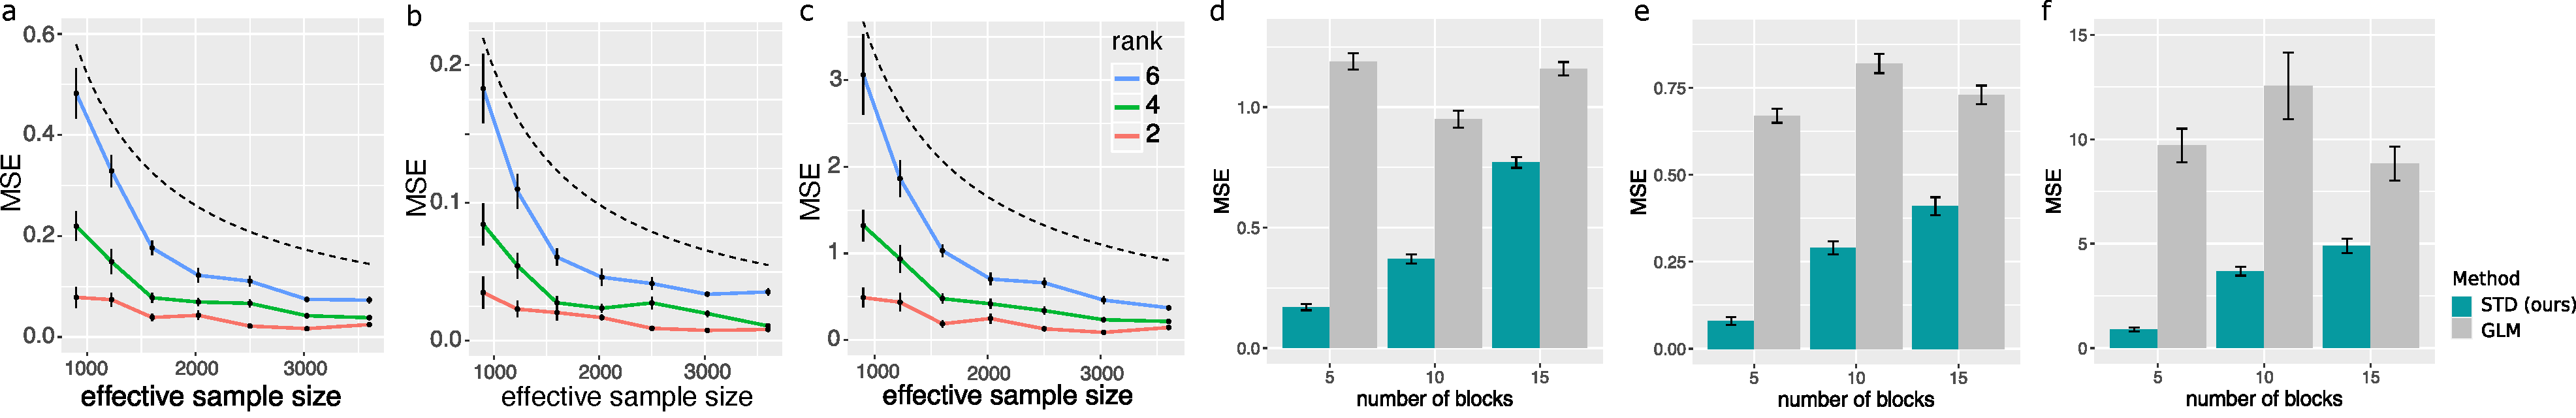
\includegraphics[width=14cm]{dim_alternative_w.pdf}
\vspace{-.5cm}
\caption{(a)-(c): Estimation error against effective sample size. The dashed curves correspond to $\tO({1/d^2})$. (d)-(f): Performance comparison under stochastic block models. The $x$-axis represents the number of blocks in the networks. The response tensors are generated from Gaussian (a, d), Poisson (b, e) and  Bernoulli  (d, f) models . }\label{fig:dim}
\end{figure}

The experiment II investigates the capability of our model in handling correlation among coefficients. We mimic the scenario of brain imaging analysis. A sample of $d_3=50$ networks are simulated, where each network measures the connections between $d_1=d_2=20$ brain nodes. We simulate $p=5$ features for the each of the 50 individuals. These features may represent, for example, age, gender, cognitive score, etc. Recent study has suggested that brain connectivity networks often exhibit community structure represented as a collection of subnetworks, and each subnetwork is comprised of a set of spatially distributed brain nodes. To accommodate this structure, we utilize the stochastic block model~\citep{abbe2017community} to generate the effect size. Specifically, we partition the nodes into $r$ blocks by assigning each node to a block with uniform probability. Edges within a same block are assumed to share the same feature effects, where the effects are drawn i.i.d.\ from $N(0,1)$. 

Figure~\ref{fig:dim}d-f compares the MSE of our method with a multiple-response GLM approach. The multiple-response GLM is to regress the dyadic edges, one at a time, on the features, and this model is repeatedly fitted for each edge. As we find in Figure~\ref{fig:dim}d-f, our tensor regression method achieves significant error reduction in all three data types considered. The outperformance is substantial in the presence of large communities; even in the less structured case ($\sim 20/15=1.33$ nodes per block), our method still outperforms GLM. The possible reason is that the multiple-response GLM approach does not account for the correlation among the edges, and suffers from overfitting. In contrast, the low-rankness in our modeling incorporates the shared information across entries.

The experiment III compares {\bf STD} with three other supervised tensor methods: Higher-order low-rank regression ({\bf HOLRR}~\cite{rabusseau2016low}), Higher-order partial least square ({\bf HOPLS}~\cite{zhao2012higher}) and Subsampled tensor projected gradient ({\bf TPG}~\cite{yu2016learning}). Figure~\ref{fig:compare} shows that {\bf STD} outperforms others, especially in the low-signal, high-rank setting. As the number of informative modes (i.e., modes with available features) increases, the {\bf STD} exhibits a substantial reduction in error whereas others remain unchanged (Figure~\ref{fig:compare}b). This showcases the benefit of incorporation of multiple features. The accuracy gain in Figure~\ref{fig:compare} demonstrates the benefit of alternating algorithm -- incorporation of informative modes also improves the estimation in the non-informative modes. 

\begin{figure}[ht]
\centering
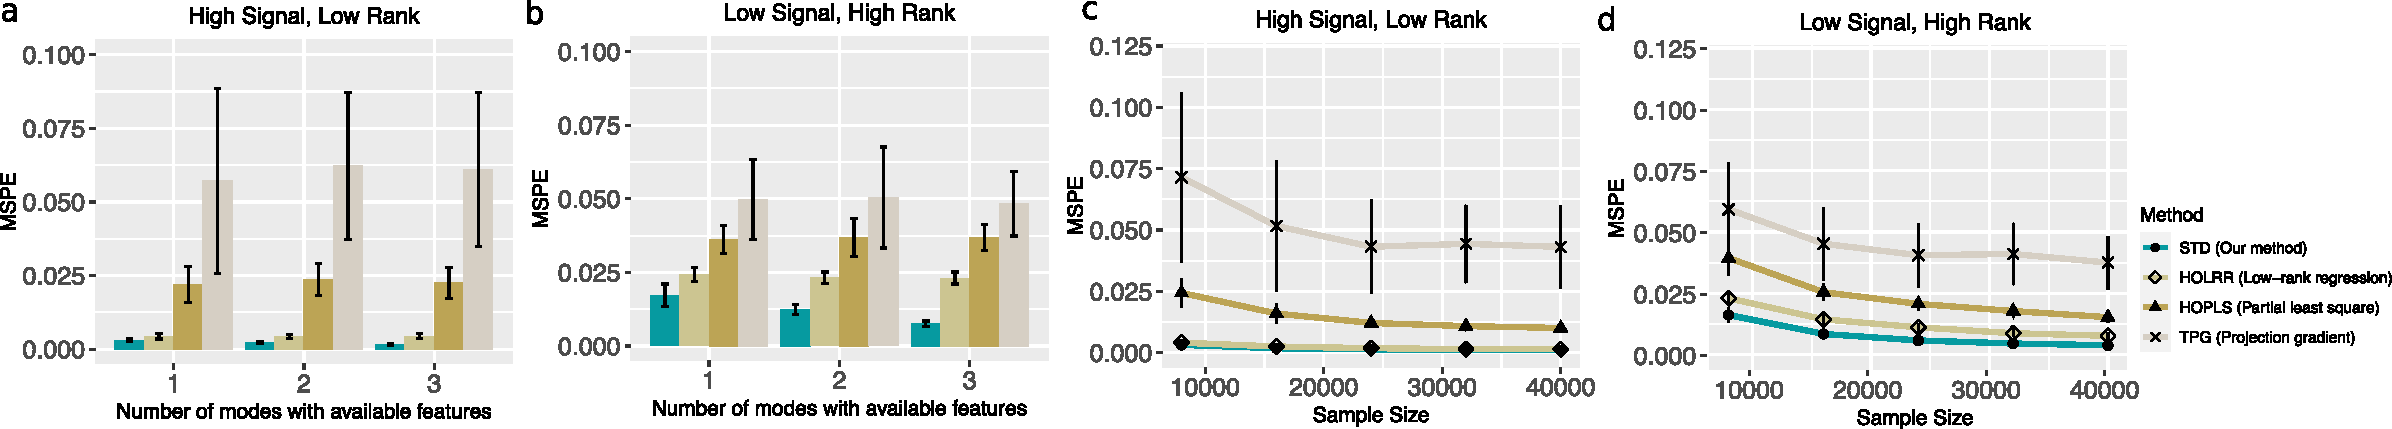
\includegraphics[width=14cm]{compare_alternative_w.pdf} 
\vspace{-.5cm}
\caption{\small Comparison between different tensor methods. Panels (a) and (b) plot mean squared prediction error (MSPE) versus the number of modes with available features. Panels (c) and (d) plot MSPE versus the effective sample size $d^2$. We consider rank $\mr=(3,3,3)$ (low) vs (4,5,6)
 (high), and signal $\alpha =3 $ (low) vs.\ 6 (high).}~\label{fig:compare}
\vspace{-.5cm}
\end{figure}



We then apply our method to brain structural connectivity networks from Human Connectome Project (HCP)~\citep{HCP}. %We analyze the structural connectivity patterns among 68 brain regions for 136 individuals from HCP. 
The dataset consists of 136 brain structural networks, one for each individual. Each brain network is represented as a 68-by-68 binary matrix, where the entries encode the presence or absence of fiber connections between the 68 brain regions. We consider four individual features: gender (65 females vs.\ 71 males), age 22-25 ($n=35$), age 26-30 ($n=58$), and age 31+ ($n=43$). The goal is to identify the connection edges that are affected by individual features. 
%A key challenge in brain network is that the edges are correlated; for example, the nodes in edges may be from a same brain region, and it is of importance to take into account the within-dyad dependence. 

\begin{figure}[!h]
\centering

\includegraphics[width=14cm]{HCP.pdf}
\vspace{-.5cm}
\caption{\small Top edges with large effects. (a) Global effect; (b) Female effect; (c) Age 22-25; (d) Age 31+. Red (blue) edges represent positive (negative) effects. Edge-widths are proportional to the magnitudes of effect sizes.
}\label{fig:brain}
\vspace{-.2cm}
%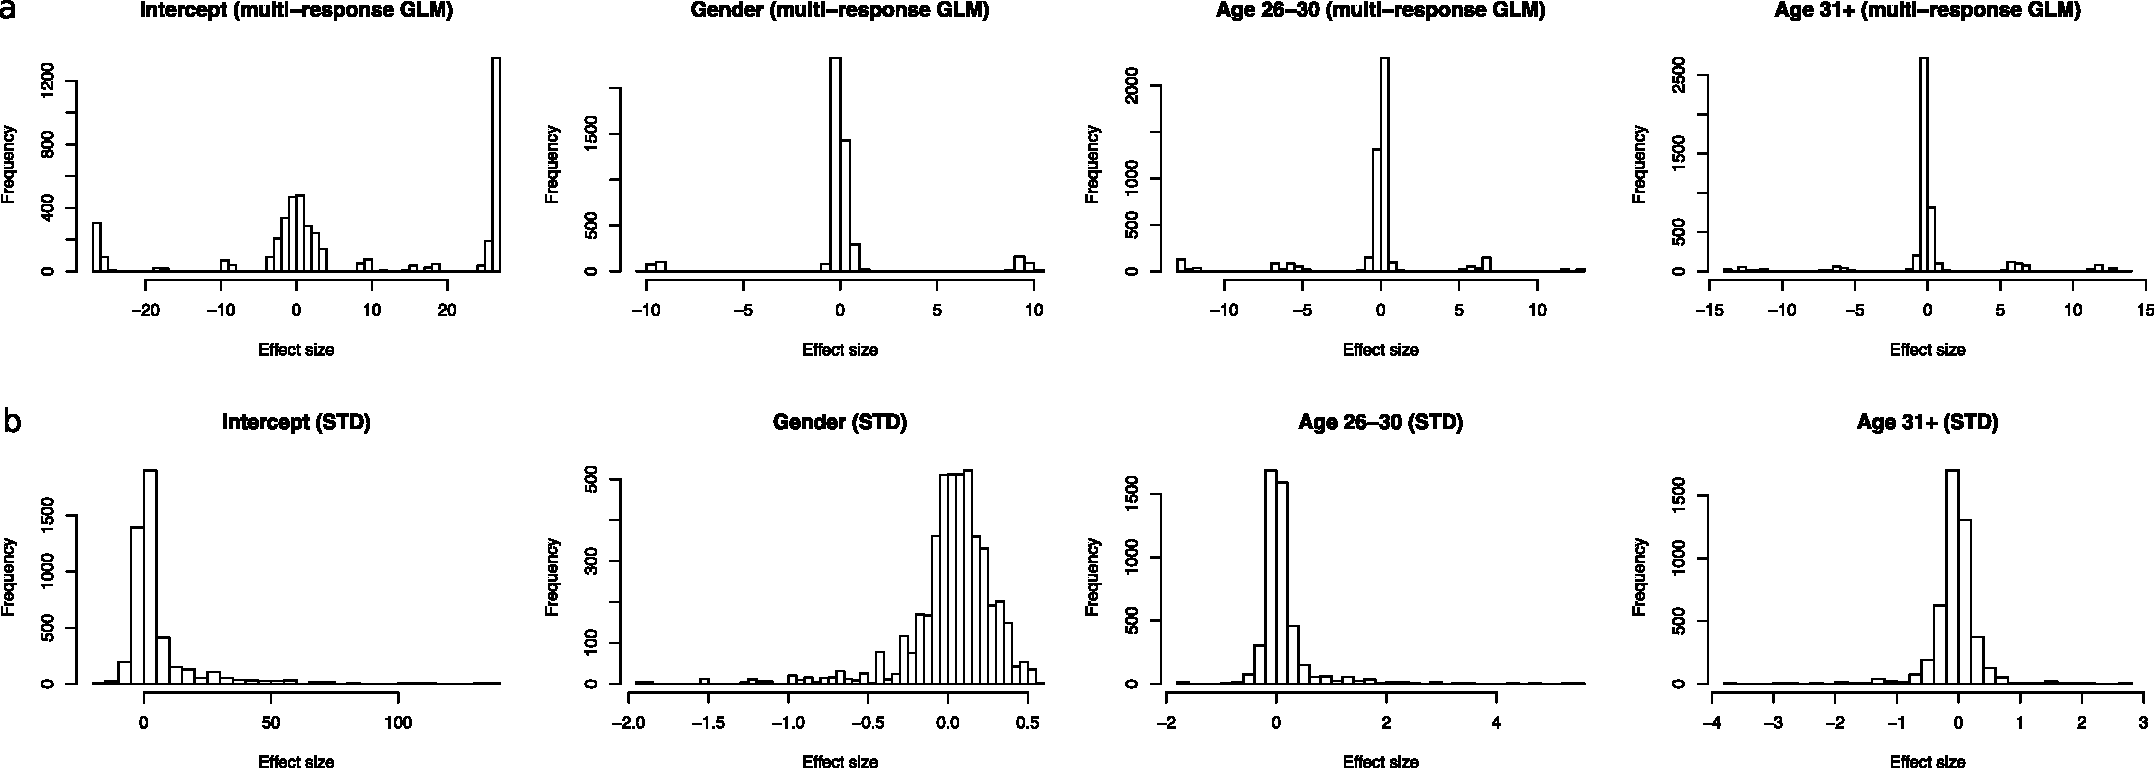
\includegraphics[width=14cm]{compare_HCP.pdf}
%\caption{Comparison of estimated feature effects the HCP data using (a) multi-response GLM and (b) supervised tensor decomposition (STD). }\label{fig:s1}
%\vspace{-.1cm}
\end{figure}


We appy the supervised tensor decomposition to the HCP data. The BIC selection suggests a rank $\mr=(10,10,4)$ with quasi log-likelihood $\tL_{\tY}=-174654.7$. Figure~\ref{fig:brain} shows the top edges with high effect size, overlaid on the Desikan atlas brain template~\citep{desikan2006automated}. We find that the global connection exhibits clear spatial separation, and that the nodes within each hemisphere are more densely connected with each other (Figure~\ref{fig:brain}a). In particular, the superior-temproal (\emph{SupT}), middle-temporal (\emph{MT}) and Insula are the top three popular nodes in the network. Interestingly, female brains display higher inter-hemispheric connectivity, especially in the frontal, parental and temporal lobes (Figure~\ref{fig:brain}b). This is in agreement with a recent study showing that female brains are optimized for inter-hemispheric communication~\citep{ingalhalikar2014sex}. We find several edges with declined connection in the group Age 31+. Those edges involve Frontal-pole (\emph{Fploe}), superior-frontal (\emph{SupF}) and Cuneus nodes. The Frontal-pole region is known for its importance in memory and cognition, and the detected decline further suggests the age effects to brain connections.


\section{Conclusion}
\vspace{-.2cm}
We have developed a supervised tensor decomposition method with side information on multiple modes. The empirical results demonstrate the improved interpretability and accuracy over previous approaches. Applications to the brain connection data yield conclusions with sensible interpretations, suggesting the practical utility of the proposed approach.

\newpage 
\section*{Broader Impact}

Our supervised tensor decomposition method is widely applicable to network analysis, dyadic data analysis, spatial-temporal model, and recommendation systems.
The new method improve the predictive power and enhance interpretability through incorporation of the interactive side information in tensor decomposition.
% We have shown the improved predictive power and enhanced interpretability by incorporating the interactive side information in tensor decomposition method.  
The application to  brain connection dataset  shows the practical utility of the proposed method.
%The application to the brain connection dataset yields conclusions with sensible interpretations, suggesting the practical utility of the proposed approach.  Tensor learning is a clear challenge for further research.
 We believe that our model enriches the research of tensor-based learning and becomes a powerful tool to boost scientific discoveries in various fields. 
%We hope the work opens up new inquiry that allows more machine learning researchers to contribute to this field.

%We have developed a supervised tensor decomposition method with side information on multiple modes. One important challenge of tensor data analysis is the complex interdependence among tensor entries and between multiple features. Our approach incorporates side information as feature matrices in the conditional mean tensor. Our empirical results demonstrate the improved interpretability and accuracy over previous approaches. The application to the brain connection dataset yields conclusions with sensible interpretations, suggesting the practical utility of the proposed approach.  We believe that our model fills the gap between theory and practice and is a powerful tool to boost scientific discoveries.

%Our exponential family tensor regression  We have shown the improved predictive power and enhanced interpretability by incorporating interactions between multiple covariate matrices. We acknowledge the opportunities and challenges in the tensor regression modeling. We hope the method developed in this paper will open up new research directions towards richer tensor-based learning. All code and data are publicly available, and we encourage members of the machine learning community to participate in these exciting problems.

\bibliography{tensor_wang}
\bibliographystyle{apalike}

\end{document}
